\documentclass[10pt,letterpaper]{article}

% -----------------------------------------------------------------------------
% SCA 2.0 position paper v3 — self-contained pdflatex source
% -----------------------------------------------------------------------------
\usepackage[margin=0.88in,top=0.82in,bottom=0.82in]{geometry}
\usepackage{mathptmx}
\usepackage[T1]{fontenc}
\usepackage{microtype}
\usepackage{amsmath,amssymb}
\usepackage{booktabs,array,tabularx}
\usepackage{graphicx}
\usepackage{tikz}
\usetikzlibrary{arrows.meta,positioning,shapes.geometric,calc}
\usepackage{xcolor}
\usepackage{hyperref}
\usepackage{enumitem}
\usepackage{titlesec}
\usepackage{caption}
\usepackage{fancyhdr}
\usepackage{multicol}

\definecolor{econblue}{RGB}{20,55,95}
\definecolor{slate}{RGB}{79,89,104}
\definecolor{mist}{RGB}{242,245,249}
\definecolor{rulegray}{RGB}{203,210,220}
\definecolor{warm}{RGB}{132,85,38}
\definecolor{green}{RGB}{42,104,78}

\hypersetup{colorlinks=true,linkcolor=econblue,citecolor=econblue,urlcolor=econblue,
  pdftitle={Synthetic Cultural Agents 2.0: Beyond Persona-Prompting},
  pdfauthor={Augusto Gonzalez-Bonorino, Kseniia Biriukova, and Monica Capra}}
\setlength{\parindent}{1.15em}
\setlength{\parskip}{0.18em}
\setlength{\headheight}{15pt}
\titlespacing*{\section}{0pt}{1.0em}{0.3em}
\titlespacing*{\subsection}{0pt}{0.68em}{0.22em}
\titleformat{\section}{\large\bfseries\color{econblue}}{\thesection.}{0.55em}{}
\titleformat{\subsection}{\normalsize\bfseries\color{econblue}}{\thesubsection}{0.45em}{}
\setlist[itemize]{leftmargin=1.3em,itemsep=0.12em,topsep=0.15em}
\setlist[enumerate]{leftmargin=1.45em,itemsep=0.12em,topsep=0.15em}
\captionsetup{font=small,labelfont={bf,color=econblue},skip=4pt}

\pagestyle{fancy}
\fancyhf{}
\fancyhead[L]{\small\color{slate} EconLLM Lab \textperiodcentered\ SCA 2.0 position paper}
\fancyhead[R]{\small\color{slate}\thepage}
\renewcommand{\headrulewidth}{0.35pt}
\renewcommand{\headrule}{\hbox to\headwidth{\color{rulegray}\leaders\hrule height \headrulewidth\hfill}}
\fancypagestyle{plain}{\fancyhf{}\fancyfoot[C]{\small\color{slate}\thepage}\renewcommand{\headrulewidth}{0pt}}

\newcommand{\SCA}{\textsc{sca}}
\newcommand{\LLM}{\textsc{llm}}
\newcommand{\DPO}{\textsc{dpo}}
\newcommand{\GPS}{\textsc{gps}}
\newcommand{\WVS}{\textsc{wvs}}
\newcommand{\WEIRD}{\textsc{weird}}
\newcommand{\cvp}{\texttt{cvprofiles}}
\newcommand{\M}{\mathcal{M}}
\newcommand{\E}{\mathbb{E}}

\begin{document}

% -----------------------------------------------------------------------------
% Cover (excluded from the paper-length target)
% -----------------------------------------------------------------------------
\thispagestyle{empty}
\begin{center}
\vspace*{1.3cm}
{\color{econblue}\rule{\textwidth}{1.15pt}}\\[0.45em]
{\LARGE\bfseries\color{econblue} Synthetic Cultural Agents 2.0:}\\[0.16em]
{\LARGE\bfseries\color{econblue} Beyond Persona-Prompting}\\[0.45em]
{\color{econblue}\rule{\textwidth}{0.55pt}}\\[0.85em]
{\large A position paper on validated AI measurement for non-\WEIRD{} populations}\\[1.0em]
{\large\textbf{Augusto Gonzalez-Bonorino}\textsuperscript{1}\quad
\textbf{Kseniia Biriukova}\textsuperscript{2}\quad
\textbf{Monica Capra}\textsuperscript{1,3}}\\[0.5em]
{\small\textsuperscript{1}Department of Economics, Arizona State University; EconLLM Lab.\\
\textsuperscript{2}EconLLM Lab.\\
\textsuperscript{3}Department of Economics, Claremont Graduate University; EconLLM Lab.}\\[0.8em]
{\normalsize August 2026 \textperiodcentered\ Working paper / position paper}\\[0.4em]
{\color{econblue}\rule{0.28\textwidth}{0.35pt}}
\end{center}

\vfill
\noindent\colorbox{mist}{\parbox{0.965\textwidth}{\small\vspace{0.25em}
\textbf{Status.} This paper sets a research standard rather than claiming that the standard has already been met. The current SCA 2.0 adapter evidence is a two-country proof of concept. It supports neither calibrated population prediction nor a general superiority claim over persona prompting. The proposed validation program is the condition for those claims. Code is available at \href{https://github.com/EconLLM-Lab/SCA2_PofW}{\texttt{github.com/EconLLM-Lab/SCA2\_PofW}}; the companion validation engine is \href{https://github.com/Bonorinoa/cvprofiles}{\texttt{cvprofiles}}.\vspace{0.25em}}}
\newpage

\section*{Statement of significance}
Many social-science questions concern people who are sparsely represented in the data used to build contemporary AI systems. Researchers increasingly fill that gap by asking a general-purpose language model to role-play a person or population. This paper argues that role prompts are useful baselines, but they are not enough for scientific simulation. We propose a different standard: treat every AI procedure that maps evidence into an outcome as a candidate measurement function; test it against independent human data and theory; and report which conclusions survive the admissible functions. Synthetic Cultural Agents 2.0 operationalizes this standard for cultural preferences by combining preference-trained open models with \cvp{}, a tool that turns construct validation into an auditable partial-identification exercise. The payoff is not a synthetic substitute for fieldwork. It is a disciplined way to generate, screen, and falsify hypotheses before scarce human data are collected.

\section*{Abstract}
Language models are now used as simulated respondents in economics, political science, and public policy. Their usual implementation, persona prompting, places a demographic or cultural description in the context window and treats the resulting answer as a population-relevant observation. That practice is fast and often useful for exploration, but it leaves the mapping from population evidence to model behavior under-specified. This paper proposes Synthetic Cultural Agents 2.0 (SCA 2.0), a research program for replacing that shortcut with validated simulation. Its first component is a family of candidate projection functions: persona prompting and retrieval-augmented prompting are contextual functions; preference fine-tuning and activation steering alter a policy before the same evaluation is applied. Its second component is \cvp{}, an open validation engine. Given a researcher-defined construct, a finite menu of candidate measures, and a preregistered nomological network, \cvp{} evaluates moment restrictions, retains the admissible measures, and reports the range of downstream conclusions across them. The framework treats validation as a design constraint, not a post-hoc score. Culture is the first application: Global Preferences Survey measures can parameterize training data for open-weight agents, while World Values Survey items, behavioral measures, and demographic patterns provide external tests. Existing two-country adapter results motivate the program but do not yet establish its central claim. The immediate task is a common benchmark that compares prompting, retrieval, fine-tuning, steering, survey composites, and simple statistical baselines on the same held-out human outcomes. If a preference-trained agent then improves on persona prompting under preregistered tests and survives construct validation, it becomes a stronger tool for hypothesis generation, questionnaire pre-piloting, and experimental design. If it fails, the same framework identifies the failure rather than converting it into a narrative.

\noindent\textit{Keywords:} AI measurement; synthetic populations; cultural preferences; construct validity; partial identification; Direct Preference Optimization; non-\WEIRD{} populations

\section{The problem: cheap simulations, weak warrants}
Social scientists have long measured latent attributes such as trust, patience, reciprocity, and risk tolerance with surveys, experiments, and behavioral traces. None of these instruments is the attribute itself. They are representations whose usefulness depends on what they preserve and what they distort. Large language models make one more representation extraordinarily cheap: a researcher can ask a model to answer as a member of a target population and obtain a synthetic sample in minutes \cite{horton2023,argyle2023,aher2023}.

This convenience changes the bottleneck. The hard question is no longer whether a researcher can generate an answer; it is whether the procedure that generated it measures anything stable about the intended population. This question is especially sharp outside the populations most visible in the data, annotator pools, and institutional settings that shape leading models. The concern is not that an AI system is ``biased'' in the abstract. It is that an unvalidated projection from a target population to an AI response can silently inherit a \WEIRD{} default, a prompt artifact, or a model-specific prior \cite{henrich2010,durmus2024}.

SCA 1.0 showed that carefully constructed persona prompts can reproduce non-\WEIRD{} patterns in economic experiments \cite{capra2025}. That result establishes persona prompting as a serious benchmark, not a straw man. But it remains a reduced-form procedure: the cultural signal is supplied in a transient context, the relevant features of that context are difficult to isolate, and a model update can change the result without changing the social-science theory. SCA 2.0 asks whether cultural variation can instead be represented in an estimable policy and then subjected to the same external discipline expected of any other measurement instrument.

\begin{figure}[t]
\centering
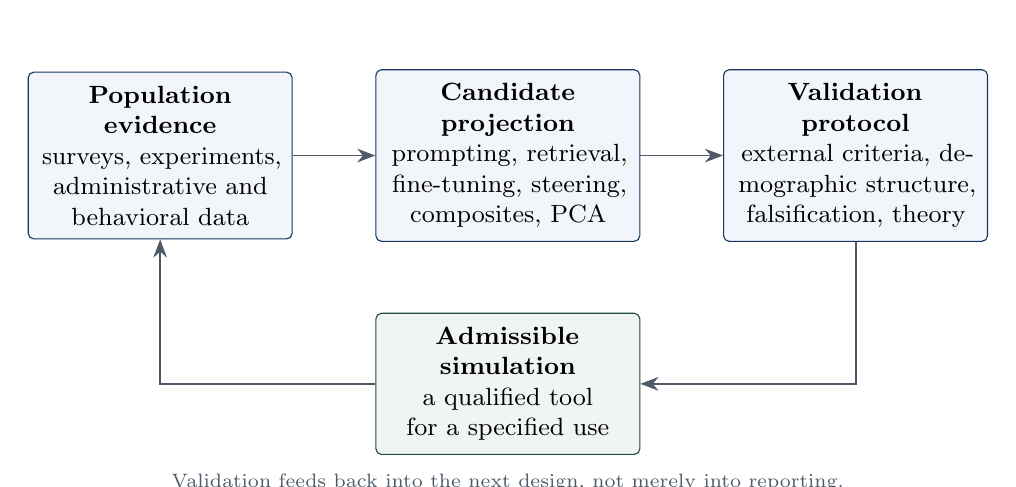
\begin{tikzpicture}[font=\small,
 box/.style={draw=econblue, rounded corners=2pt, fill=mist, align=center, text width=3.0cm, minimum height=1.0cm, inner sep=5pt},
 validbox/.style={draw=green!75!black, rounded corners=2pt, fill=green!7, align=center, text width=3.0cm, minimum height=1.0cm, inner sep=5pt},
 arr/.style={-{Stealth[length=2.3mm]}, line width=.7pt, color=slate}]
\node[box] (evidence) {\textbf{Population evidence}\\surveys, experiments, administrative and behavioral data};
\node[box, right=1.05cm of evidence] (function) {\textbf{Candidate projection}\\prompting, retrieval, fine-tuning, steering, composites, PCA};
\node[box, right=1.05cm of function] (test) {\textbf{Validation protocol}\\external criteria, demographic structure, falsification, theory};
\node[validbox, below=0.9cm of function] (output) {\textbf{Admissible simulation}\\a qualified tool for a specified use};
\draw[arr] (evidence)--(function);
\draw[arr] (function)--(test);
\draw[arr] (test.south) |- (output.east);
\draw[arr] (output.west) -| (evidence.south);
\node[font=\scriptsize\color{slate},below=.12cm of output] {Validation feeds back into the next design, not merely into reporting.};
\end{tikzpicture}
\caption{The proposed research loop. A simulation is not validated by sounding plausible or by agreeing with another AI system. It earns a limited use claim only after a prespecified projection function survives external and theoretical tests.}
\label{fig:loop}
\end{figure}

\clearpage
\section{A general framework for validated AI measurement}
\subsection{Projection functions, not one privileged method}
Let $X$ denote evidence about a target population and let $Y$ be an outcome relevant to a scientific question. A procedure $m_j$ maps available inputs into a score, choice distribution, or simulated response: $m_j(X)$. We call $m_j$ a \emph{projection function}. The term is deliberately broader than ``model.'' It includes a survey composite, a principal component, an experimental outcome, and an AI-based procedure.

The distinction among AI procedures still matters. Persona prompting and retrieval-augmented generation are \emph{contextual projections}: they leave the policy fixed and change the information supplied at inference. Fine-tuning and activation steering are \emph{policy interventions}: they change the policy whose responses are later scored. In all four cases, the object that enters an empirical analysis is the evaluated output $m_j(X)$, so each belongs in the same measurement menu. Calling them all ``measurement'' is accurate only in this downstream sense; it should not obscure their different causal and engineering properties.

For SCA 2.0, the menu should be explicit before results are inspected:
\[
\M=\{m_{\mathrm{persona}},m_{\mathrm{RAG}},m_{\mathrm{base}},m_{\mathrm{DPO}},m_{\mathrm{steer}},m_{\mathrm{composite}},m_{\mathrm{PCA}},m_{\mathrm{experiment}}\}.
\]
The last three entries are crucial. A DPO agent should not be compared only with other LLMs. Survey composites and PCA are transparent statistical alternatives; incentivized experimental measures and held-out human survey outcomes provide different-method criteria. Agreement among several prompted models is not construct validity because their errors may be correlated \cite{campbell1959,ludwig2026}.

\subsection{Validation as partial identification}
Construct validity asks whether a score can support a stated interpretation. Cronbach and Meehl's answer was a \emph{nomological network}: a valid measure should bear theoretically specified relations to other observables \cite{cronbach1955}. The framework below converts that idea into an auditable decision rule.

A researcher defines a construct $C$, a finite menu $\M$, auxiliary observables $V$, and restrictions $r\in\mathcal{R}$. Each restriction has a literature-anchored threshold $\theta_r$:
\begin{equation}
 r:\qquad \E\left[g_r\{m_j(X),V;\theta_r\}\right]\geq 0.
 \label{eq:restriction}
\end{equation}
The sample analogue $s_r(m_j)$ is the restriction's slack. With tolerance $\delta\geq0$, the admissible measures are
\begin{equation}
 \M^*=\left\{m_j\in\M:s_r(m_j)\geq-\delta\quad \forall r\in\mathcal{R}\right\}.
 \label{eq:admissible}
\end{equation}
For a downstream target $\beta(m)$, such as a treatment-effect estimate or correlation with an economic outcome, the honest estimand is not automatically a single number. It is the construct-identified set
\begin{equation}
 \mathcal{B}^*=\{\beta(m):m\in\M^*\},\qquad [L,U]=[\min\mathcal{B}^*,\max\mathcal{B}^*].
 \label{eq:range}
\end{equation}
This is partial identification: data and stated assumptions determine a set of conclusions, not more \cite{manski2003,schennach2021}. \cvp{} implements this sequence---score, restrict, identify, report---with frozen inputs, a full slack profile, bootstrap uncertainty over units, and threshold-sensitivity diagnostics. It does not choose the construct or write the network. Those remain the researcher's responsibility.

Passing these restrictions means that a measure is consistent with the nominated network. It does not prove that the latent attribute causes the score, that the construct is uniquely defined, or that the policy can answer arbitrary questions about a population \cite{borsboom2004}. Empty admissible sets and wide ranges are useful outcomes: they tell the researcher that the current evidence does not warrant the intended interpretation.

\subsection{From validation to an autoresearch loop}
The framework permits a feedback loop, but only after a clear separation between evaluation and optimization. Let $z$ be a target cultural state, let $q(z)$ generate preference-training pairs, and let $\pi_\theta$ be an open-weight policy trained on those pairs. A validation profile $\mathcal{V}(\pi_\theta)$ can screen the resulting output against preregistered restrictions. The next training design may then change the data generator, regularization, or policy-intervention strength and repeat the evaluation on held-out data.

This is a constrained research loop, not self-confirmation:
\[
\text{theory and human evidence}\;\rightarrow\;q(z)\;\rightarrow\;\pi_\theta\;\rightarrow\;\mathcal{V}(\pi_\theta)\;\rightarrow\;\text{revised design}.
\]
Training directly on the same validation moments would turn the loop into benchmark fitting. A credible implementation needs a locked network, distinct development and test criteria, negative controls, and a frozen final evaluation. Under those conditions, one can ask a meaningful question such as: among policies trained to express GPS trust, which ones also preserve externally observed trust relations? This is the route by which validation may discipline alignment to a latent construct.

\section{SCA 2.0: culture as the first application}
\subsection{Structural conjecture and design}
The Global Preferences Survey supplies cross-country measures of patience, risk taking, positive and negative reciprocity, altruism, and trust \cite{falk2018}. SCA 2.0 uses a country's six-dimensional profile $z_c$ to label country-neutral preference scenarios. Direct Preference Optimization then adjusts an open-weight student policy so that preferred responses are more likely than rejected responses relative to a reference policy \cite{rafailov2023}. Under the Bradley--Terry interpretation, DPO estimates relative reward margins, not a cardinal human utility function \cite{bradley1952}.

The structural conjecture is deliberately narrow: a policy trained on preference pairs generated from $z_c$ may encode enough of the intended directional disposition to improve a prespecified human-outcome criterion without country information in its evaluation prompt. It does \emph{not} assert that the agent ``is Mexican,'' that the six GPS coordinates exhaust culture, or that policy changes identify causal cultural effects. Varying labels in a synthetic training distribution is a controlled intervention on the model, not a randomized intervention on people.

\begin{figure}[t]
\centering
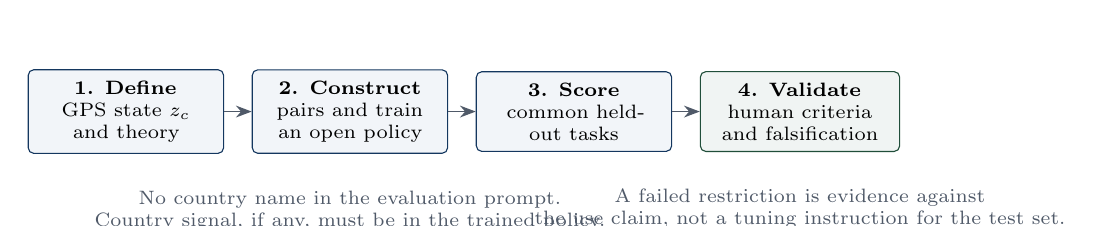
\begin{tikzpicture}[font=\scriptsize,
 box/.style={draw=econblue, rounded corners=2pt, fill=mist, align=center, text width=2.20cm, minimum height=.9cm, inner sep=4pt},
 check/.style={draw=green!75!black, rounded corners=2pt, fill=green!7, align=center, text width=2.25cm, minimum height=.9cm, inner sep=4pt},
 arr/.style={-{Stealth[length=2mm]}, line width=.65pt, color=slate}]
\node[box] (gps) {\textbf{1. Define}\\GPS state $z_c$ and theory};
\node[box, right=.35cm of gps] (train) {\textbf{2. Construct}\\pairs and train an open policy};
\node[box, right=.35cm of train] (score) {\textbf{3. Score}\\common held-out tasks};
\node[check, right=.35cm of score] (valid) {\textbf{4. Validate}\\human criteria and falsification};
\draw[arr] (gps)--(train); \draw[arr] (train)--(score); \draw[arr] (score)--(valid);
\node[font=\scriptsize\color{slate},align=center,below=.35cm of train] {No country name in the evaluation prompt.\\Country signal, if any, must be in the trained policy.};
\node[font=\scriptsize\color{slate},align=center,below=.35cm of valid] {A failed restriction is evidence against\\the use claim, not a tuning instruction for the test set.};
\end{tikzpicture}
\caption{SCA 2.0 as a specific instance of the general framework. Training is only the middle of the argument; validation determines the permitted interpretation.}
\label{fig:sca}
\end{figure}

\subsection{The current evidence and its proper role}
The existing pipeline has completed a useful but limited proof of concept. On 35 unseen WVS Wave 7 items, the Mexico adapter's fixed option distribution was closer to Mexican survey responses than the US adapter's on 34 items; the USA adapter degraded fit relative to the base model on both US and Mexican data. Because country labels were omitted at evaluation, these outcomes are consistent with country-specific information being represented in the adapter weights. They do not establish country-conditioned inference, calibrated response shares, or an explanation for the US degradation. Option scoring also showed under-dispersion relative to human response distributions.

These findings should motivate the benchmark; they should not carry the paper's general claim. In particular, a two-country comparison cannot demonstrate that DPO dominates persona prompting, because persona prompting and retrieval have not yet been evaluated on the same preregistered outcomes. Nor should a training-pair recovery score be treated as validity evidence, since it shares generative ancestry with the training labels. The compact evidence profile and the trust illustration are reported in Appendix~A as examples of the reporting standard, rather than as the paper's main result.

\section{What would justify the claim? A common evaluation program}
The program's decisive test is not another isolated adapter result. It is a common benchmark in which all candidate projections answer the same held-out tasks, are compared with the same human reference, and face the same negative controls. Table~\ref{tab:matrix} gives the required design.

\begin{table}[t]
\centering
\small
\caption{Minimum common evaluation matrix. A check mark means that the method must be evaluated on that surface, not that it is expected to pass.}
\label{tab:matrix}
\begin{tabularx}{\textwidth}{@{}>{\raggedright\arraybackslash}p{2.25cm} c c c c >{\raggedright\arraybackslash}X@{}}
\toprule
\textbf{Candidate} & \textbf{OOS items} & \textbf{Human criterion} & \textbf{Demographic structure} & \textbf{Placebos} & \textbf{Interpretation if it passes}\\
\midrule
Persona prompt & \checkmark & \checkmark & \checkmark & \checkmark & Reduced-form baseline\\
RAG prompt & \checkmark & \checkmark & \checkmark & \checkmark & Evidence-sensitive contextual baseline\\
DPO adapter & \checkmark & \checkmark & \checkmark & \checkmark & Candidate policy-level projection\\
Steering & \checkmark & \checkmark & \checkmark & \checkmark & Candidate controllable projection\\
Composite / PCA & \checkmark & \checkmark & \checkmark & \checkmark & Transparent non-LLM comparator\\
Experiment & --- & \checkmark & \checkmark & \checkmark & Different-method anchor\\
\bottomrule
\end{tabularx}
\end{table}

The benchmark must include at least four resolutions. First, compare country-level criterion recovery while reporting uncertainty and sensitivity to development covariates. Second, test demographic gradients within countries, where a measure must reproduce predeclared signs and magnitudes rather than merely country means. Third, compare cell means after within-country demeaning. Fourth, evaluate response distributions on items that were never used for training, prompt construction, retrieval, or measure selection. These resolutions answer different failure modes; no single correlation can replace them.

The comparator family must also be broader than LLM variants. A survey composite and PCA can outperform an elaborate agent on some outcomes; that is a substantive result, not an embarrassment. Conversely, a DPO agent that passes where a prompt fails may be useful precisely because the policy intervention produces a more stable projection. The expected outcome is a qualified frontier, not a universal ranking.

A credible superiority claim would therefore read: \emph{for a predeclared construct, population, task family, and external criteria, method $m_{\mathrm{DPO}}$ achieved better performance than persona prompting and the named alternatives, while satisfying the locked validity restrictions.} The word ``better'' must be attached to this design. It should not be used before the comparison is run.

\section{Research uses, boundaries, and release strategy}
If the benchmark supports the narrow claim above, SCA 2.0 can support several uses. It can help researchers generate hypotheses, stress-test draft questionnaires, and select between candidate instruments before fieldwork. With a construct-identified effect range, it can support power calculations across defensible effect sizes instead of relying on a single convenient prior. It may assist in piloting field or laboratory interventions by identifying questions and behavioral margins worth measuring. These uses remain subordinate to human data; the agent proposes and screens, while fieldwork adjudicates.

Three uses are not supported by the present design: polling or forecasting absolute population shares, individual-level diagnosis, and causal counterfactual claims about people. The last boundary matters. A validated agent may provide a model-based counterfactual of its own policy under a controlled intervention. That does not identify the human causal response absent an independently defensible bridge.

\subsection{Necessary extensions before a general-science submission}
A serious PNAS- or Nature-facing manuscript needs more than a polished account of two adapters. The minimum package is:
\begin{enumerate}
\item \textbf{Validate the target constructs first.} Lock construct definitions, measurement menus, thresholds, and negative controls before interpreting adapter outcomes. Expand the trust-style profile into multi-restriction networks for each GPS dimension; report empty sets where the current WVS bridge fails.
\item \textbf{Run the common benchmark.} Add persona prompting immediately and retrieval-augmented prompting where data provenance permits. Include DPO, steering, base models, survey composites, PCA, and a different-method human anchor. Pre-register the scoring and aggregation rules.
\item \textbf{Broaden the panel and its variation.} Add countries selected to span GPS profiles, linguistic settings, and baseline-model proximity; use independent survey sources where coverage allows; and reserve countries, questions, and constructs that are untouched until final evaluation.
\item \textbf{Test robustness and falsification.} Vary base models, seeds, prompt templates, item wording, calibration procedures, and training-data size. Add deliberately invalid measures, shuffled-country labels, and mismatched constructs. Report failures alongside successes.
\item \textbf{Make the artifact auditable.} Release frozen protocols, score tables where licenses permit, code, model cards, data documentation, and reproducible figures. The public claim should be reconstructible without access to private reasoning or a proprietary API.
\end{enumerate}

Open release on Hugging Face should follow, not precede, these gates. The appropriate near-term decision is \emph{release readiness}, not a premature public adapter launch: document base-model and survey licenses, remove any restricted training material, publish a model card with the permitted use claim and known failures, version the evaluation suite, and archive the exact adapter and protocol hashes. Once those conditions are met, a gated or fully public Hugging Face release is a scientific asset because it allows independent replication. Before then, an adapter download can invite stronger uses than the evidence warrants.

\section{Conclusion}
The central wager of SCA 2.0 is not that a fine-tuned language model can replace respondents. It is that social science can use AI-generated simulations more carefully than it has used generic persona prompts: by treating prompts, retrieval systems, trained policies, steering interventions, and conventional composites as competing projection functions; by testing them against a researcher-authored validity network and independent human evidence; and by reporting the set of conclusions that survives.

Culture provides a demanding first case because the relevant attributes are latent, the populations are heterogeneous, and the temptation to substitute a plausible narrative for a measurement argument is strong. SCA 2.0 combines a way to construct policy-level candidates with a way to reject them. If that combination yields a reproducible improvement over prompting, it will support a new kind of validated simulation for non-\WEIRD{} populations. If it does not, the result is still valuable: it marks the boundary of what current synthetic agents can responsibly claim.

\appendix
\section{Illustrative reporting standard: two compact evidence profiles}
This appendix records the current evidence in its proper place. It is not a substitute for the common benchmark proposed above.

\subsection{Adapter proof of concept}
Figure~\ref{fig:adapter} visualizes the present two-country result. The matched Mexico adapter beat the cross-country adapter on 34 of 35 held-out WVS questions, with mean $\Delta\mathrm{TVD}=0.1495$ and a 95\% interval $[0.0964,0.2152]$. In the US comparison, the USA adapter fit worse than both the base model and the Mexico adapter. These are distributional-alignment results for fixed outputs under unconditioned prompts, not evidence that the agent infers country at test time.

\begin{figure}[h]
\centering
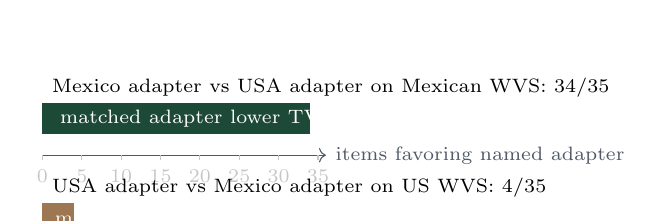
\begin{tikzpicture}[x=0.10cm,y=0.55cm,font=\scriptsize]
\draw[->,color=slate] (0,0)--(36,0) node[right]{items favoring named adapter};
\foreach \x in {0,5,...,35} \draw[gray!45] (\x,0)--(\x,-.12) node[below]{\x};
\fill[green!70!black] (0,.5) rectangle (34,1.2);
\node[anchor=west] at (0,1.55) {Mexico adapter vs USA adapter on Mexican WVS: $34/35$};
\node[anchor=west,text=white] at (1,0.85) {matched adapter lower TVD};
\fill[warm!80] (0,-1.8) rectangle (4,-1.1);
\node[anchor=west] at (0,-.75) {USA adapter vs Mexico adapter on US WVS: $4/35$};
\node[anchor=west,text=white] at (.35,-1.45) {matched};
\end{tikzpicture}
\caption{Current adapter evidence, expressed as the item-level matched-versus-cross comparison. The figure is intentionally descriptive: it does not provide a cross-method benchmark or identify a mechanism.}
\label{fig:adapter}
\end{figure}

\subsection{Why a validity layer changes the analysis}
A frozen country-level trust profile compares four WVS trust facets to GPS trust across 42 overlapping countries. At the prespecified correlation floor of $0.30$, generalized trust Q57 has $r=0.278$ and is rejected; in-group, out-group, and institutional facets have $r=0.349$, $0.303$, and $0.332$. The three-facet survivor composite has $r=0.410$. This example does not crown a universal trust measure. It shows that a familiar single item and a composite can support materially different measurement claims.

\begin{figure}[h]
\centering
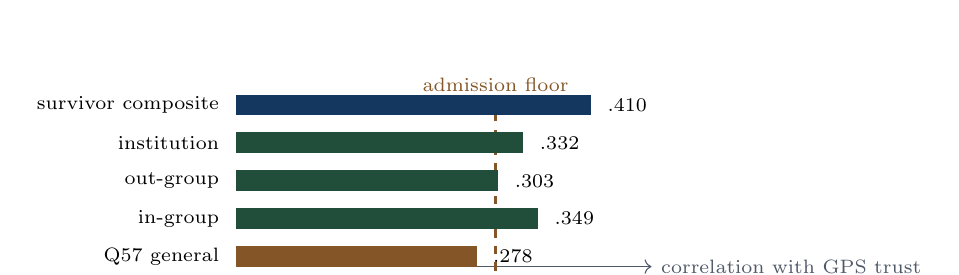
\begin{tikzpicture}[x=11cm,y=.48cm,font=\scriptsize]
\draw[->,color=slate] (0,0)--(.48,0) node[right]{correlation with GPS trust};
\draw[dashed,thick,color=warm] (.30,-.55)--(.30,4.35) node[above,text=warm]{admission floor};
\foreach \y/\lab/\val/\col in {0/{Q57 general}/.278/warm,1/{in-group}/.349/green!75!black,2/{out-group}/.303/green!75!black,3/{institution}/.332/green!75!black,4/{survivor composite}/.410/econblue} {
  \fill[\col] (0,\y) rectangle (\val,\y+.55);
  \node[anchor=east] at (-.008,\y+.27) {\lab};
  \node[anchor=west] at (\val+.008,\y+.27) {\val};}
\end{tikzpicture}
\caption{Illustrative trust validity profile. This is one convergent restriction, not a complete validation argument; the proposed program adds demographic, discriminant, known-groups, and falsification restrictions.}
\label{fig:trust}
\end{figure}

\section{Operational details of \cvp{}}
The validation engine receives a unit-by-measure score table, a researcher-authored network, a target functional, a seed, and a versioned protocol. It returns the slack for every measure-restriction pair, the admissible set, the image of the target over that set, bootstrap uncertainty over units, and a threshold grid. Run identifiers hash frozen inputs so that an output can be traced to the exact score table and protocol. The tool has no language-model calls and does not infer the researcher's theory. This separation makes it suitable both for SCA 2.0 and for non-AI measurement problems.

\begin{thebibliography}{99}\small
\bibitem{aher2023} Aher, G., R. I. Arriaga, and A. T. Kalai (2023). ``Using Large Language Models to Simulate Multiple Humans and Replicate Human Subject Studies.'' \textit{ICML}.
\bibitem{argyle2023} Argyle, L. P., E. C. Busby, N. Fulda, J. R. Gubler, C. Rytting, and E. S. Wiley (2023). ``Out of One, Many: Using Language Models to Simulate Human Samples.'' \textit{Political Analysis} 31(3): 337--351.
\bibitem{borsboom2004} Borsboom, D., G. J. Mellenbergh, and J. van Heerden (2004). ``The Concept of Validity.'' \textit{Psychological Review} 111(4): 1061--1071.
\bibitem{bradley1952} Bradley, R. A., and M. E. Terry (1952). ``Rank Analysis of Incomplete Block Designs: I. The Method of Paired Comparisons.'' \textit{Biometrika} 39: 324--345.
\bibitem{campbell1959} Campbell, D. T., and D. W. Fiske (1959). ``Convergent and Discriminant Validation by the Multitrait-Multimethod Matrix.'' \textit{Psychological Bulletin} 56: 81--105.
\bibitem{capra2025} Capra, C. M., A. Gonzalez-Bonorino, and M. Pantoja (2025). ``LLMs Can Model Non-WEIRD Populations: Experiments with Synthetic Cultural Agents.'' Forthcoming, \textit{Review of Experimental Economics}.
\bibitem{cronbach1955} Cronbach, L. J., and P. E. Meehl (1955). ``Construct Validity in Psychological Tests.'' \textit{Psychological Bulletin} 52: 281--302.
\bibitem{cvprofiles} EconLLM Lab / A. Gonzalez-Bonorino (2026). \texttt{cvprofiles}: Construct-Validity Profiles. \url{https://github.com/Bonorinoa/cvprofiles}.
\bibitem{durmus2024} Durmus, E., et al. (2024). ``Towards Measuring the Representation of Subjective Global Opinions in Language Models.'' \textit{COLM}.
\bibitem{falk2018} Falk, A., A. Becker, T. Dohmen, B. Enke, D. Huffman, and U. Sunde (2018). ``Global Evidence on Economic Preferences.'' \textit{Quarterly Journal of Economics} 133: 1645--1692.
\bibitem{henrich2010} Henrich, J., S. J. Heine, and A. Norenzayan (2010). ``The Weirdest People in the World?'' \textit{Behavioral and Brain Sciences} 33: 61--83.
\bibitem{horton2023} Horton, J. J. (2023). ``Large Language Models as Simulated Economic Agents: What Can We Learn from Homo Silicus?'' NBER Working Paper 31122.
\bibitem{ludwig2026} Ludwig, J., S. Mullainathan, and A. Rambachan (2026). ``Large Language Models: An Applied Econometric Framework.'' \textit{Annual Review of Economics} 18.
\bibitem{manski2003} Manski, C. F. (2003). \textit{Partial Identification of Probability Distributions}. Springer.
\bibitem{rafailov2023} Rafailov, R., A. Sharma, E. Mitchell, S. Ermon, C. D. Manning, and C. Finn (2023). ``Direct Preference Optimization: Your Language Model is Secretly a Reward Model.'' \textit{NeurIPS}.
\bibitem{schennach2021} Schennach, S. M. (2021). ``Measurement Systems.'' cemmap Working Paper CWP12/21.
\end{thebibliography}
\end{document}
